\documentclass{article}
\usepackage[utf8]{inputenc}
\usepackage{graphicx}
\usepackage[colorlinks=true, allcolors=black]{hyperref}
\usepackage{listings}
\usepackage[a4paper, total={6in, 8in}]{geometry}
\usepackage{pdfpages}
\usepackage{float}
\usepackage{soul}
\usepackage{multicol}
\usepackage{multirow}
\usepackage[section]{placeins}
\usepackage[
backend=biber,
sorting=none]{biblatex}

\graphicspath{ {./img/} }

\addbibresource{bibliography.bib}

\lstset{
  basicstyle=\ttfamily,
  columns=fullflexible,
  breaklines=true,
}

\NewDocumentCommand{\codeword}{v}{%
\texttt{\textcolor{black}{#1}}%
}

\title{CS5011: P2 - Machine Learning}
\author{190018035}
\date{March 13th 2024}

% PAGE LIMIT: 10, including text, figures, tables

\begin{document}

\maketitle

\tableofcontents

\section{Introduction}
% Include checklist of parts completed & extension
For this practical, I was tasked with implementing and evaluating different machine learning models on the Pump It Up: Data Mining the Water Table \cite{DrivenData} dataset. This involved experimenting with different preprocessing steps, hyperparameters, and machine learning models to find the best model to predict the status of water pumps in Tanzania. The checklist below details my achievements in the practical for each of the specified parts.

\subsection{Project Achievements}
\begin{itemize}
    \item{Part 1: Attempted and Fully Working}
    \item{Part 2: Attempted and Fully Working}
\end{itemize}

\subsection{Usage Instructions}

To run the script, navigate to the root directory and run the following command:

\begin{lstlisting}[language=bash]
python3 part1.py <train-input-file> <train-labels-file> <test-input-file> <numerical-preprocessing> <categorical-preprocessing> <model-type> <test-prediction-output-file>
\end{lstlisting}

\noindent The values for each of the arguments are equivalent to that described in the assignment specification. However, one difference is that the \codeword{<numerical-preprocessing>} and \codeword{<categorical-preprocessing>} arguments now take in a \codeword{Manual} option, which allows features to be preprocessed based on the encoding that are most suitable for the model. 

\section{Part 1}
In this section, I will detail the various preprocessing steps I took to prepare the data for the machine learning models, guided by a deep exploration of the dataset. I will also discuss the design decisions I made while implementing this part, including the parameters of the preprocessing methods and the hyper-parameters of the machine learning models.

\subsection{Preprocessing Steps}
Prior to implementing the machine learning models, I performed a number of preprocessing steps to clean and prepare the data for the models. These steps were guided by a deep exploration of the dataset, where I analyzed the distribution of the features, the relationships between the features, and other important characteristics of the dataset. In conjuction with the steps outlined below, I will also discuss my findings from the exploration that lead to the decisions I made.

\subsubsection{Cleaning the Data}
The following steps were taken to clean the data:

\paragraph{Removing Irrelevant Features}
The first step I took was to remove any features that were irrelevant to the prediction task. These features either did not directly contribute to the status of the water pumps or contained too many missing values. The features that were removed include:

\begin{itemize}
  \item \codeword{id} The identifier for the water pump is not relevant to the prediction task
  \item \codeword{wpt_name} The name of the water pump is unlikely to contribute to the prediction task
  \item \codeword{scheme_name} The name of the water scheme is unlikely to contribute to the prediction task
  \item \codeword{num_private} This feature contains mostly missing values, with over 99.24\% of the values missing (defined as 0). Additionally, the feature does not have a clear definition, so it is unclear how it would contribute to the prediction task.
  \item \codeword{amount_tsh} Similarly, this feature contains mostly missing values, with over 70.1\% of the values missing (also defined as 0). 
\end{itemize}

\paragraph{Removing Single-Value Features}
I also removed any features that only contained a single value, as they do not contribute to the prediction task. There was only one feature that met this criteria, which was \codeword{recorded_by}.

\paragraph{Removing Redundant Features}
There were a number of features that were redundant, meaning they contained the same information as another feature. I removed these features to reduce the dimensionality of the dataset. There were a few considerations I made when deciding which of the features that are redundant to remove. The first consideration was the cardinality of the feature - having too many unique values would make the feature difficult to encode, whilst having too few unique values would make the feature less informative. The second consideration was the number of missing values in the feature - if a feature had a large number of missing values, it would be less informative. The features that were removed include:

\begin{itemize}
  \item \codeword{payment} This feature contains the same information as \codeword{payment_type} with the same value counts, so I removed it and retained \codeword{payment_type}.
  \item \codeword{quantity} Similarly, this feature contains the same information as \codeword{quantity_group} with the same value counts, so I removed it and retained \codeword{quantity_group}.
  \item \codeword{extraction_type} This feaure was removed in favor of \codeword{extraction_type_group} and \\ \codeword{extraction_type_class}. The \codeword{extraction_type_class} feature provides a more general classification of the extraction type. It contains only 7 unique values, which makes it easier to encode, and the smallest value count for a given category for this feature is 117. The \codeword{extraction_type_group} feature, on the other hand, contains 13 unique values, where the smallest value count for a given category is 98. Finally, the \codeword{extraction_type} feature contains 18 unique values, where the smallest value count for a given category is 2. From this information, we can see that the \codeword{extraction_type_class} feature is the most general, and the \codeword{extraction_type} feature is the most specific. In order to provide more useful information to the model, I decided to remove the \codeword{extraction_type} feature and retain the other two, as this feature has the highest cardinality with the smallest value count for a given category whilst the other two features have a lower cardinality with a higher value count for a given category, thereby providing more useful information to the model.
  \item \codeword{scheme_management} This feature was removed in favor of \codeword{management}. These two features contain most of the same categories; however, the \codeword{scheme_management} feature contains 3878 missing/unknown values whereas management only contains 561 unknown values. This makes the \codeword{management} feature more informative and easier to encode, so I decided to remove the \codeword{scheme_management} feature.
  \item \codeword{water_quality} This feature was removed in favor of \codeword{quality_group}. These two features contain mostly the same information, where \codeword{water_quality} splits "salty" and "flouride" into two subcategories (introducing a "salty abandoned" and "flouride abandoned" subcategory). These subcategories contain comparatively few values, so I decided to remove the \codeword{water_quality} feature and retain the \codeword{quality_group} feature to reduce the dimensionality of the dataset.
  \item \codeword{source} This feature was removed in favor of \codeword{source_type} and \codeword{source_class}. The \codeword{source_class} feature is the most general, containing only 3 unique values, and the \codeword{source_type} feature sits in the middle, containing 7 unique values and containing very similar columns to \codeword{source}. The \codeword{source} feature contains 10 unique values. Since \codeword{source_class} provides the most general information, and since \codeword{source} contains the highest cardinality, I decided to remove the \codeword{source} feature and retain the other two so there is a balance between the general and specific information provided to the model.
  \item \codeword{waterpoint_type_group} This feature was removed in favor of \codeword{waterpoint_type}. The \\ \codeword{waterpoint_type} splits up the "communal standpipe" category into "communal standpipe" and "communal standpipe multiple". However, since "communal standpipe multiple" only contains contains relatively few values (6103), I decided to remove the \codeword{waterpoint_type_group} feature and retain the \codeword{waterpoint_type} feature to reduce the dimensionality of the dataset.
\end{itemize}

\paragraph{Replacing Construction Year with Decades}
The \codeword{construction_year} feature contained a large number of missing values, with 34.8\% of the values missing. To make the feature more informative, I decided to categorize the construction years into decades. This would allow the model to learn the relationship between the construction year and the status of the water pumps, without imputing values that might distort the underlying distribution of the data. The decades were defined from 1960s to the 2010s, with the missing values being replaced with the "Unknown" category.

% TODO REDO
\paragraph{Imputing Missing Values}
When dealing with the categorical features, I replaced the missing values with the "Unknown" category. However, when it came to dealing with numerical features, a key consideration was whether to impute the missing values or to remove the rows with missing values. I decided to impute the missing values with the median of the feature based on the region. This decision was made after analyzing the distribution of the features and finding that the features contained a large number of outliers. Imputing the missing values with the median would be less sensitive to the outliers and would not distort the underlying distribution of the data.

% TODO REDO
\paragraph{Fixing Formatting Issues}
When exploring the \codeword{funder} and \codeword{installer} features, I found that there were a large number of unique values that were the same but were formatted differently. For example, "Government Of Tanzania" and "Government of Tanzania" were the same entity but were formatted differently. To deal with this, I converted the values to lowercase and removed any leading/trailing whitespace. I then performed a fuzzy matching algorithm to identify the unique values that were the same but were formatted differently. I then replaced the values with the same unique value. This strategy reduced the number of unique values for each of the features, making the dataset more manageable.

\paragraph{Limiting High Cardinality Features}
There were a few features in the dataset, specifically \codeword{funder}, \codeword{installer}, \codework{subvillage} and \codeword{ward}, that contained a large number of unique values. Such high cardinality could pose challenges, as encoding these features could significantly increase the dimensionality of the dataset, potentially leading to issues like overfitting and increased computational demand. To address this, I set a threshold (95\%) that identifies the most frequent categories that cumulatively account for 95\% of the values in the feature. This threshold was determined through manual experimentation, but can be set through hyperparameter optimization. Through this strategy, I was able to reduce the number of dummy variables needed for encoding and makng the dataset size more manageable. The remaining categories were replaced with the "Other" category. Additionally, I also replaced the missing values with the "Unknown" category. This strategy resulted in the following reductions in the number of unique values for each of the features (after fixing formatting issues):

\begin{table}[H]
\centering
\begin{tabular}{|c|c|c|}
\hline
\textbf{Feature} & \textbf{Original Unique Values} & \textbf{Reduced Unique Values} \\ \hline
\codeword{funder} & 1883 & 405 \\ \hline
\codeword{installer} & 1905 & 397 \\ \hline
\codeword{subvillage} & 19287 & 16336 \\ \hline
\codeword{ward} & 2092 & 1578 \\ \hline
\end{tabular}
\caption{Reduction in Unique Values for High Cardinality Features}
\end{table}

% TODO REDO
\paragraph{Converting Datetime Features}
The

\subsubsection{Encoding the Data}

\subsection{Design Decisions}

\subsection{Evaluation}

\begin{table}[]
\begin{tabular}{|l|l|l|l|l|l|l|}
\hline
\textbf{}              & SS + OHE & SS + Ord & SS + Target & PT + OHE & PT + Ord & PT + Target \\ \hline
Random Forest          & 80.74\%  & 80.79\%  & 80.4\%      & 80.2\%   & 79.09\%  & 79.85\%     \\ \hline
Logistic Regression    & 78.49\%  & 62.24\%  & 75.52\%     & 78.37\%  & 61.44\%  & 75.53\%     \\ \hline
Gradient Boosting      & 75.96\%  & 75.16\%  & 77.53\%     & 75.71\%  & 74.56\%  & 74.56\%     \\ \hline
Hist Gradient Boosting & 79.39\%  & 79.12\%  & 79.62\%     & 78.67\%  & 78.37\%  & 78.89\%     \\ \hline
MLP                    & 77.59\%  & 53.36\%  & 78.16\%     & 77.54\%  & 54.33\%  & 77.7\%      \\ \hline
\end{tabular}
\end{table}

\section{Part 2}
% Analyse the results of your experiments based on the provided training set (via cross-
% validation mechanism). Summarise the key insights and findings of your analysis.
For this part of the practical, I utilized Optuna \cite{optuna_2019}, an automated hyper-parameter optimization (HPO) tool to find the best hyper-parameters for each of the models. In this section, I will detail my HPO process and analyze the results of the experiments.

% TODO REDO
\subsection{Hyper-Parameter Optimization}
I decided to use Optuna to perform the hyper-parameter optimization for the Random Forest and Logistic Regression models. I chose Random Forest as from the previous part, it was the best performing model, and Logistic Regression as it is a simple model that can be used as a benchmark. I also wanted to see how HPO differs for different families of models. The hyper-parameters that I optimized for each of the models are detailed below.

% TODO REDO
\subsubsection{Random Forest}
When running the study for the Random Forest model, I optimized the following hyper-parameters:

\begin{itemize}
  \item \codeword{n_estimators} The number of trees in the forest
  \item \codeword{max_depth} The maximum depth of the tree
  \item \codeword{min_samples_split} The minimum number of samples required to split an internal node
  \item \codeword{min_samples_leaf} The minimum number of samples required to be at a leaf node
  \item \codeword{max_features} The number of features to consider when looking for the best splits
\end{itemize}

% TODO REDO
\subsubsection{Logistic Regression}
When running the study for the Logistic Regression model, I optimized the following hyper-parameters:

\begin{itemize}
  \item \codeword{C} Inverse of regularization strength
  \item \codeword{penalty} The norm used in the penalization
  \item \codeword{solver} The algorithm to use in the optimization problem
  \item \codeword{class_weight} Weights associated with classes in the form \{class\_label: weight\}
  \item \codeword{tol} Maximum number of iterations taken for the solvers to converge
  \item \codeword{max_iter} Maximum number of iterations taken for the solvers to converge
\end{itemize}

\subsection{Evaluation}

\subsubsection{Random Forest}
When running the trials, I found that the most important hyper-parameters for the Random Forest model were \codeword{cat_encoder}, \codeword{max_depth}, and \codeword{max_features}. These parameters were the most influential in determining the performance of the model. 

\begin{figure}[H]
  \centering
  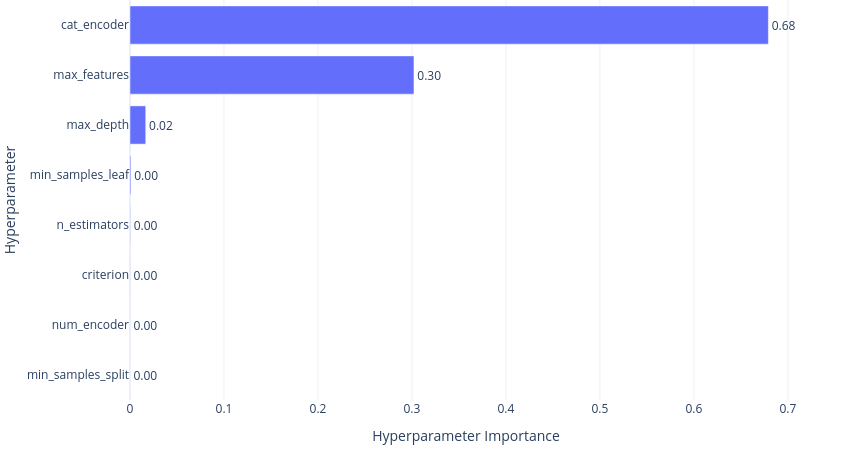
\includegraphics[width=0.8\textwidth]{img/random_forest_importance.png}
  \caption{Feature Importance for Random Forest Model}
\end{figure}

\noindent In addition, the parallel coordinates plot for the Random Forest model for the most influential features is shown below.

\begin{figure}[H]
  \centering
  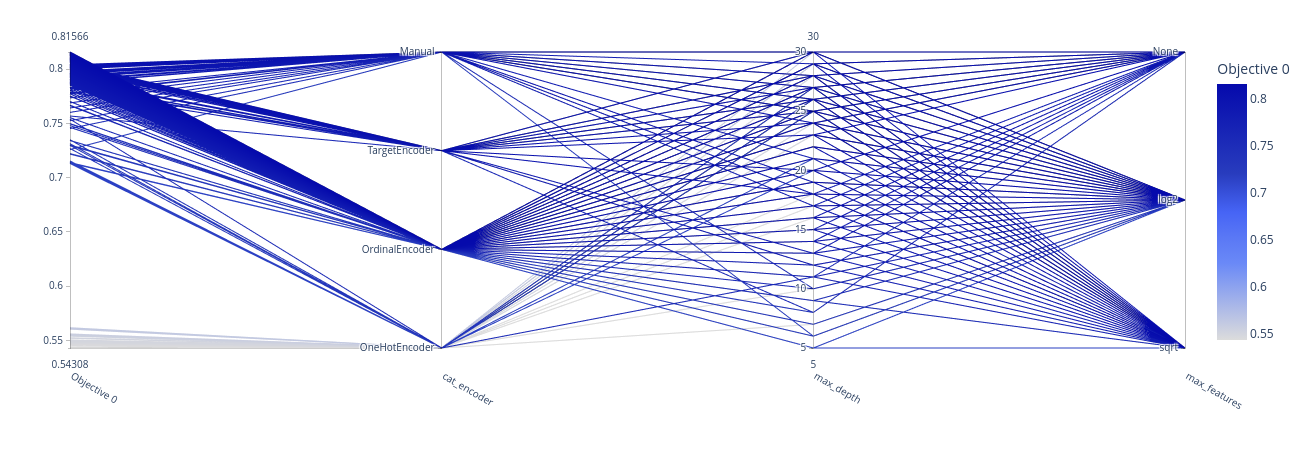
\includegraphics[width=0.8\textwidth]{img/tmp.png}
  \caption{Parallel Coordinates Plot for Random Forest Model}
\end{figure}

\subsubsection{Logistic Regression}
When running the trials, I found that the most important hyper-parameters for the Logistic Regression model were \codeword{cat_encoder}, \codeword{solver}, and \codeword{class_weight}. These parameters were the most influential in determining the performance of the model.

\begin{figure}[H]
  \centering
  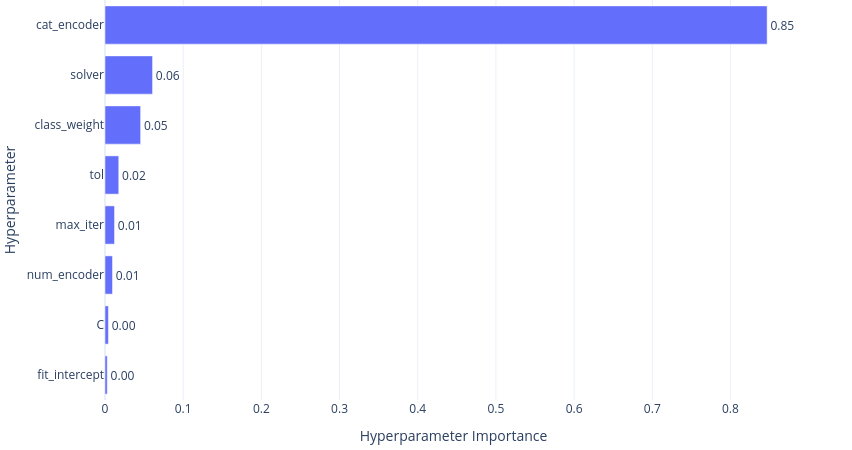
\includegraphics[width=0.8\textwidth]{img/lr_importance.png}
  \caption{Feature Importance for Logistic Regression Model}
\end{figure}

\noindent In addition, the parallel coordinates plot for the Logistic Regression model for the most iinfluencial features is shown below.

\begin{figure}[H]
  \centering
  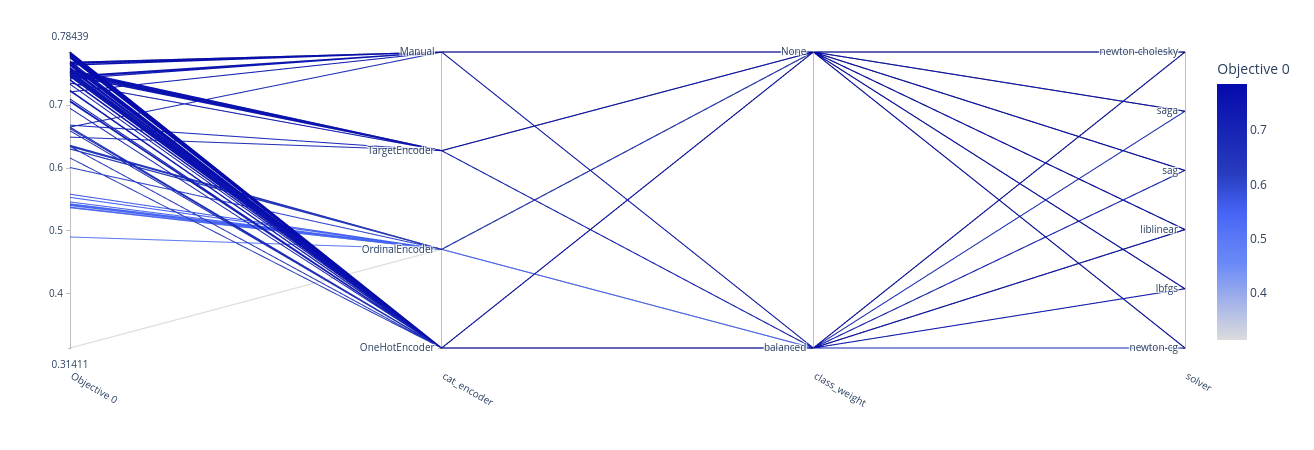
\includegraphics[width=0.8\textwidth]{img/tmp2.png}
  \caption{Parallel Coordinates Plot for Logistic Regression Model}
\end{figure}

% \section{Conclusion}

\printbibliography

\end{document}
